\documentclass[12pt]{article}
\usepackage{amsmath,amssymb}
\usepackage{cite}
\usepackage[utf8]{inputenc}
\usepackage{rotating}
\usepackage[english]{babel}
\usepackage[T1]{fontenc}
\usepackage{color}
\usepackage{xcolor}
\usepackage{textcomp}
\usepackage{indentfirst}
\usepackage{array}
\usepackage{titlesec}
\usepackage{float}
\usepackage{listings}
\usepackage{listingsutf8}
\usepackage{natbib}
\usepackage{url}
\usepackage{graphicx}
%\graphicspath{{images/}}
\usepackage{parskip}
\usepackage{fancyhdr}
\usepackage{vmargin}
\usepackage[utf8]{inputenc}
\usepackage[T1]{fontenc}
\usepackage{gensymb}

\usepackage{verbatim}
\usepackage{subfigure}
\usepackage{algorithmic}
\usepackage{framed}
\usepackage{rotating}
\usepackage{cite}
\usepackage{enumitem}
\usepackage{scrextend}
\usepackage{textcomp}

\newcommand{\subsubsubsection}[1]{\paragraph{#1}\mbox{}\\}

\setmarginsrb{3 cm}{2.5 cm}{3 cm}{2.5 cm}{1 cm}{1.5 cm}{1 cm}{1.5 cm}
\setlength{\parindent}{2em}
\setlength{\parskip}{0em}
\titleformat{\chapter}{\bfseries\Large}{\arabic{chapter}.~}{0pt}{}
\addto\captionsenglish{
  \renewcommand{\contentsname}
    {Index}
}
\newlist{nota}{enumerate}{1}
\setlist[nota]{label=Nota: ,leftmargin=*, font=\bfseries}

\definecolor{pythonred}{rgb}{0.6,0,0} % strings
\definecolor{pythongreen}{rgb}{0.25,0.5,0.35} % comments
\definecolor{pythonpurple}{rgb}{0,0.35,0.35} % keywords
\definecolor{pythonblue}{rgb}{0.25,0.35,0.75} % javadoc

\lstdefinestyle{Python}{
inputencoding=utf8/latin1,
language=python
}

\lstdefinestyle{bash}{
inputencoding=utf8/latin1,
language=bash
}

\lstset{
inputencoding=utf8/latin1,
breaklines=true,
basicstyle=\ttfamily\small,
keywordstyle=\color{pythonpurple}\bfseries,
stringstyle=\color{pythonred},
commentstyle=\color{pythongreen},
morecomment=[s][\color{pythonblue}]{/**}{*/},
numbers=none,
numberstyle=\tiny\color{black},
stepnumber=1,
numbersep=10pt,
tabsize=3,
showspaces=false,
showstringspaces=false,
moredelim=**[is][\color{orange}]{?}{?},
moredelim=**[is][\color{red}]{*}{*},
extendedchars=true,
literate=
{á}{{\'a}}1
{à}{{\`a}}1
{ã}{{\~a}}1
{é}{{\'e}}1
{è}{{\`e}}1
{ê}{{\^e}}1
{í}{{\'i}}1
{ó}{{\'o}}1
{õ}{{\~o}}1
{ú}{{\'u}}1
{ü}{{\"u}}1
{ç}{{\c{c}}}1
}


\title{\LARGE Physical Distancing Detector
\\ \vspace{5mm}
\\ \large using the OpenCV and OpenPose Python libraries}

\makeatletter
\let\thetitle\@title
\let\theauthor\@author
\let\thedate\@date
\makeatother

\pagestyle{fancy}
\fancyhf{}
\rhead{Paula Mihalcea}
\lhead{Physical Distancing Detector}
\cfoot{\thepage}

\begin{document}

%%%%%%%%%%%%%%%%%%%%%%%%%%%%%%%%%%%%%%%%%%%%%%%%%%%%%%%%%%%%%%%%%%%%%%%%%%%%%%%%%%%%%%%%%

\begin{titlepage}
	\centering
    \vspace*{0.5 cm}
    
\includegraphics[scale = 0.85]{img/logo.jpg}\\[1.0 cm]

	\textsc{\LARGE Ingegneria Informatica}\\[2 cm]	
	\rule{\linewidth}{0.2 mm} \\[0.4 cm]
	{ \huge \bfseries \thetitle}\\
	\rule{\linewidth}{0.2 mm} \\[1 cm]

	\textsc{\large Image and Video Analysis}\\[1 cm]
	\begin{minipage}{0.4\textwidth}
		\begin{flushleft} \large
			\emph{Professor:}\\
			Pietro Pala\\
            		%\normalsize{Info su\\
            		%dipartimento\\
            		%del docente}\\
			\end{flushleft}
			\end{minipage}~
			\begin{minipage}{0.4\textwidth}
        
		\begin{flushright} \large
			\emph{Student:} \\
			Paula Mihalcea\\
		\end{flushright}
        
	\end{minipage}\\[2 cm]
	
	\vspace*{2.8 cm}
	\begin{center} \large
			June - July 2020
		\end{center}
	
\end{titlepage}

%%%%%%%%%%%%%%%%%%%%%%%%%%%%%%%%%%%%%%%%%%%%%%%%%%%%%%%%%%%%%%%%%%%%%%%%%%%%%%%%%%%%%%%%%

\tableofcontents
\pagebreak

%%%%%%%%%%%%%%%%%%%%%%%%%%%%%%%%%%%%%%%%%%%%%%%%%%%%%%%%%%%%%%%%%%%%%%%%%%%%%%%%%%%%%%%%%

\begin{abstract}
   This paper presents a Python program that, through the use of the OpenCV\cite{cvpython} and OpenPose\cite{oppython} libraries, is able to process a video stream and detect if any of the people present in each frame are violating the physical distancing safety measures imposed by the 2020 COVID-19 pandemic. Although the OpenPose library is rather resource demanding (thus cannot be executed on any device), the software has been built with a real-world application in mind, and written with many practical measures meant to ease its setup and use for the average user.
\end{abstract}

%%%%%%%%% BODY TEXT
\section{Introduction}
\label{chap:intro}

The year 2020 will certainly be remembered for the spread of COVID-19, a virus which gravely affected both the global economy and our daily lives. From the lockdowns that many countries imposed to their citizens to the mandatory use of masks, many measures have been taken in order to contain its rapid transmission; among these efforts we can find various regulations that require people to keep a minimum distance of about 1.8 – 2.00 meters among them, particularly in public areas.

The problem with the last measure is that, unlike the others, there is no easy way to correctly carry it out without having at least an idea about how long two meters are. It might seem trivial, but not everyone has a good sense of measure, and estimating the correct distance to keep from others might prove quite difficult for some.

\begin{figure}[H]
\begin{center}
    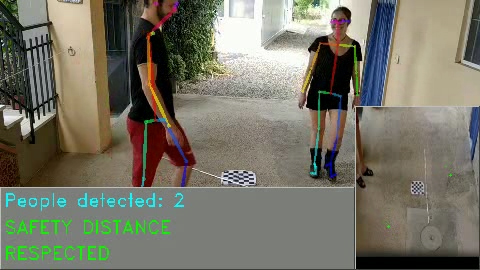
\includegraphics[width=0.85\linewidth]{img/sample_c2_1.jpg}
\end{center}
   \caption{Two people that are respecting the safety distance.}
\label{fig:c21}
\end{figure}

\begin{figure}[H]
\begin{center}
    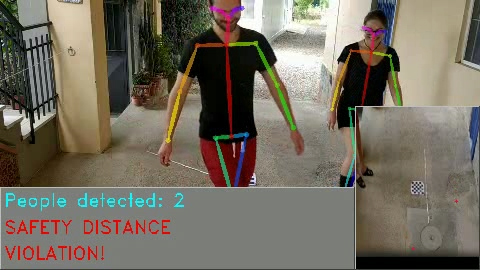
\includegraphics[width=0.85\linewidth]{img/sample_c2_2.jpg}
\end{center}
   \caption{The same people from fig. \ref{fig:c21} are not respecting that distance anymore.}
\label{fig:c22}
\end{figure}

The idea behind the software presented in this paper is to offer a tool that can automatically measure the distance between two or more people and warn them if they are too close. It also shows a map that displays their position, providing said people with a way to better understand how much two meters (or any other safety distance is provided to the program) actually measure.

%-------------------------------------------------------------------------
\section{Operating principles}
\label{chap:principles}
The program simply takes an input video stream (webcam or file) and overlays on every frame a status bar which informs about the number of people detected in said frame and whether they are respecting or not a given safety physical distance\footnote{From now on this distance will always be assumed to be equal to 2 meters.}. Along with this information is displayed a (partial) view from above of the visible floor, on which the estimated position of the detected people is marked with colored dots. An external \lstinline{INI} file can be used to set up and customize almost every aspect of the program, from the appearance of the status bar to the dimensions of the map in pixels and meters.

\subsection{Information needed}
\label{chap:info}
Depending on the information available about the environment framed in the video, the program needs different data to be able to properly create the map.

In the worst-case scenario, it only needs the length of the sides of a rectangular mat that can be laid on the floor framed in the video and used to determine the dimensions of the area around it. Otherwise, if such a mat is not available, the user will have to specify at least the width and height of the visible portion of floor (or the desired part that is going to be selected).

\subsubsection{Source points (corners)}
\label{chap:srcpts}
In addition to this, since the geometric transformations used to create the map need at least four points in the video to work (the corners\footnote{These corners will also interchangeably be called \textit{points} from now on.} of the visible floor or the mat), the user might also want to specify them in pixel coordinates for better precision; this is especially true in low resolution videos where a few pixels can make the difference between a good and a bad transformation (see figures \ref{fig:nopixels} and \ref{fig:pixels}).

\begin{figure}[H]
  \centering
  \begin{minipage}[b]{0.45\textwidth}
    \centering
    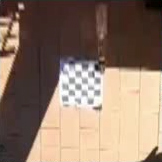
\includegraphics[width=3cm,keepaspectratio]{img/no_pixels.jpg}
    \caption{Map created with mat source points carefully extracted and saved in the setup file.}
    \label{fig:nopixels}
  \end{minipage}
  \hfill
  \begin{minipage}[b]{0.45\textwidth}
    \centering
    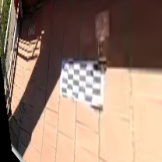
\includegraphics[width=3cm,keepaspectratio]{img/pixels.png}
    \caption{Map created with hand-picked mat source points; it is visibly less accurate.}
    \label{fig:pixels}
  \end{minipage}
\end{figure}

However, if these coordinates cannot be obtained prior to initialization, the program will prompt the user with the first frame extracted from the video and ask him or her to click directly on the image to determine them automatically. Technically, this method is as effective as specifying the points in the setup file, but in practice it is more prone to error as selecting the corners with a mouse is usually less precise than writing the actual accurate coordinates.

\subsection{Assumptions}
\label{chap:assumptions}
An important assumption needed for the program to work correctly is that the area framed by the camera does not change during execution (for example by moving the camera), as the map is created during the initialization phase and cannot be edited afterwards, if not by stopping the program and initializing it again.

\subsection{Workflow}
\label{chap:workflow}
After starting the program with a valid input source, which can be done by writing in a terminal opened in the main folder (\lstinline{Physical distancing detector}) the following command\footnote{See chapter \ref{chap:main} for details about the command line arguments.}:
\begin{lstlisting}[style=bash]
python3 physical_distancing_detector.py source [save] [destination] [setup_file]
\end{lstlisting}
the main script will check if the setup file already contains any reference corners in the form of pixel coordinates.

\subsubsection{Corners detection}
\label{chap:corners}
The possibility to specify these corners directly in the \lstinline{INI} file was meant to ease the setup for those users that have a fixed camera and possess (almost) complete knowledge about the environment it has been installed in, in addition to improve accuracy. If corners are specified for both a mat and the visible floor, the program will ask the user which ones it should use to generate the map. Otherwise, as mentioned above, for those who do not know said points, it will prompt a window containing the first frame of the video, in order to allow the user to choose the corners by clicking on them then pressing \lstinline{ENTER} (fig. \ref{fig:chessselection}).

\begin{figure}[H]
\begin{center}
    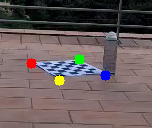
\includegraphics[width=0.3\linewidth]{img/chess_selection.jpg}
\end{center}
   \caption{Mat corners selection window with all four points selected.}
\label{fig:chessselection}
\end{figure}

\subsubsubsection{Additional borders}
\label{chap:borders}
It is worth mentioning that if the user chooses to manually select the floor corners the program gives him or her the possibility to add a border to the image, in order to be able to generate a more accurate map by also selecting points that might fall outside the visible frame (see figures \ref{fig:floor} and \ref{fig:borders}). This option is available by simply pressing \lstinline{SPACEBAR} while in floor corners selection mode, then entering the desired thickness of the borders in pixels (fig. \ref{fig:bordersterminal}).

\begin{figure}[H]
  \centering
  \begin{minipage}[b]{0.45\textwidth}
    \centering
    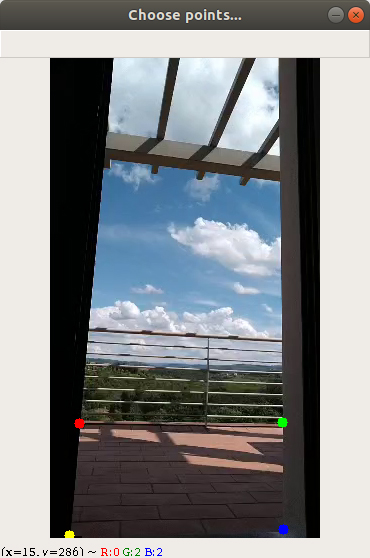
\includegraphics[height=5cm,keepaspectratio]{img/floor_selection.jpg}
    \caption{Source points selection window without additional borders.}
    \label{fig:floor}
  \end{minipage}
  \hfill
  \begin{minipage}[b]{0.45\textwidth}
    \centering
    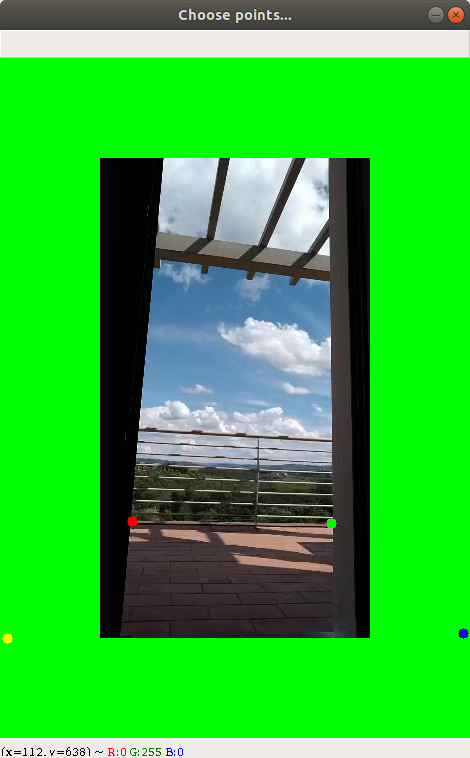
\includegraphics[height=5cm,keepaspectratio]{img/borders.png}
    \caption{Source points selection window with 100px green borders.}
    \label{fig:borders}
  \end{minipage}
\end{figure}

\begin{figure}[H]
\begin{center}
    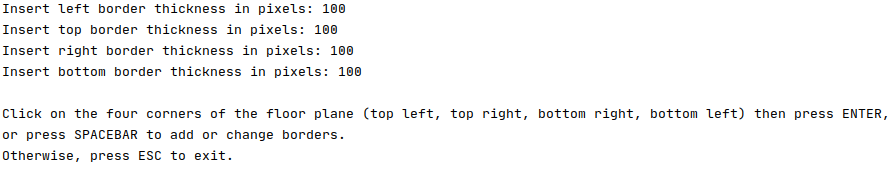
\includegraphics[height=0.18\linewidth]{img/borders_terminal.png}
\end{center}
   \caption{Insertion of border thickness in the terminal.}
\label{fig:bordersterminal}
\end{figure}

\subsubsection{Map generation}
\label{chap:map}
After getting the four corners (in a way or another), the program proceeds with the map generation by applying a homography to the quadrangle obtained by connecting the points. The four destination points for the homography (see \ref{chap:homography}) can either be determined automatically (as in the case of the mat, or of the floor if no other points are available) or also specified by the user in the setup file (again, this usually yields a better map in the floor setup, particularly for irregular views, as shown in figures \ref{fig:notgood} and \ref{fig:good}).

\begin{figure}[H]
  \centering
  \begin{minipage}[b]{0.45\textwidth}
    \centering
    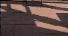
\includegraphics[width=2.8cm,keepaspectratio]{img/auto_map.jpg}
    \caption{Map created with automatically calculated destination points; perspective clearly isn't perfect.}
    \label{fig:notgood}
  \end{minipage}
  \hfill
  \begin{minipage}[b]{0.45\textwidth}
    \centering
    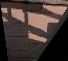
\includegraphics[width=2.8cm,keepaspectratio]{img/nice_map.jpg}
    \caption{Map created using user-specified destination points; perspective looks way better.}
    \label{fig:good}
  \end{minipage}
\end{figure}

The map and the homography matrix generated during this step are saved for later use: the map for the video overlay, the matrix for determining the position of the people detected in the video.

\subsubsection{Video processing}
\label{chap:processing}
The program thus proceeds with feeding each video frame to the OpenPose library, which analyses it and returns the keypoints of the people it detects in it. By elaborating the heel keypoints and applying the homography matrix to their coordinates, the program determines the position of a person and prints it on the map, while also informing the user about possible violations of the physical safety distance.

From this point on, the program runs indefinitely or until the source video file reaches the end; it can be safely closed by pressing \lstinline{ESC}.

%-------------------------------------------------------------------------

\section{Technical details}
\label{chap:tech}
The program, written in the Python programming language, makes use of mainly two libraries: OpenCV for the video processing and map creation and OpenPose for detecting any people present in a given scene.

It is made of many components, of which the \lstinline{physical_distancing_detector.py} script is the main one. In this section they will be analyzed one by one in order of appearance and somewhat importance.

%---------------------------------

\subsection{Main program}
\label{chap:main}
This script contains the main function, and can be executed from the terminal with the following arguments:
\begin{itemize}
\item \lstinline{source}: the video stream source; can be a file or \lstinline{0} for the webcam;
\item \lstinline{save} \textit{(optional)}: can be \lstinline{True} or \lstinline{False}; it specifies whether the processed video should be saved on disk;
\item \lstinline{destination} \textit{(optional)}: if the processed video is going to be saved, the user can specify the output file name with this argument (otherwise the system will assign an appropriate one);
\item \lstinline{setup_file} \textit{(optional)}: specifies the \lstinline{INI} file to be used during initialization, if different from the default one (\lstinline{setup.ini}); useful if the user has many different cameras or setups.
\end{itemize}

As mentioned in section \ref{chap:corners}, this script reads the \lstinline{INI} file to load all the needed parameters and checks if there are any reference points saved in there, then proceeds as explained in said paragraph. It uses a \lstinline{mode} flag (\lstinline{True} for floor corners, \lstinline{False} for mat) in order to determine, in each subsequent function, which coordinates should be used (floor or mat), since the transformations needed for the two mechanisms are different.

The script then opens the given video stream by using the OpenCV \lstinline{VideoCapture()} method\cite{cvcamera}; since this function is sometimes prone to error, the script will make a certain number of attempts\footnote{Specified in the setup file under the \lstinline{max_attempts} parameter.} to open it before returning an error and exiting.

After eventually creating an OpenCV \lstinline{VideoWriter} object to save the processed video (if the \lstinline{save} argument was \lstinline{True}), the program passes the first frame to \lstinline{process_frame_first()}, thus delegating to this function the map generation, then proceeds to feed the subsequent frames to the similar \lstinline{process_frame()} function, in a loop.

Once the video has ended, or the user has chosen to exit the program by pressing \lstinline{ESC}, the script safely exists by saving the video to disk (if needed) and closing the video window before exiting.

%---------------------------------

\subsection{Setup}
\label{chap:setup}
The \lstinline{read_ini.py} script unifies the parsing of the \lstinline{setup.ini} file in a single function, in order to better process the data it contains; it stores these parameters in a series of “themed” dictionaries (\lstinline{system}, \lstinline{map}, \lstinline{mat}, \lstinline{overlay} and \lstinline{status bar}) in order to access only once the disk for the settings' retrieval. For this purpose, the file also contains a few utility functions to process some data types found in the \lstinline{INI}, such as colors and point coordinates.

Even though the setup file provided with the program contains adequate default values for all parameters, a complete explanation of all variables therein present is given within the \lstinline{read_ini.py} file itself.

%---------------------------------

\subsection{Frame processing}
\label{chap:frameprocess}
As the name suggests, this script contains the two functions needed for the complete processing of each video frame, including the OpenPose application (it begins with the import of precisely this library - and throws an error if it does not find it).

\subsubsection{\textit{process\_frame\_first()}}
\label{chap:processframefirst}
The \lstinline{process_frame_first()} function takes in input many parameters from the main function, of which the most important are the OpenCV \lstinline{VideoCapture} and \lstinline{VideoWriter} objects, the \lstinline{mode} flag and many settings read from the \lstinline{INI} file.

After checking the validity of the video frame that has read, it calls the \lstinline{get_points()} function\footnote{Found in the \lstinline{get_points.py} script.} in order to set the reference points needed for the homography, then the \lstinline{generate_overlay()} function\footnote{\label{overlaynote}Found in the \lstinline{overlay.py} script.} for the map and status bar generation.

The \lstinline{process_frame_first()} function proceeds by calculating and setting a few other parameters further needed, then gets the keypoints of the detected people by using the OpenPose library. It then gives these keypoints, along with other data from the dictionaries previously created by the \lstinline{read_ini()} function, to the \lstinline{transform_coords()} function\footnote{Found in the homonymous script.}, in order to obtain the position on the map of each person and if there are any distance violations. The script proceeds with applying the overlay on the frame through the \lstinline{apply_overlay()} function\footref{overlaynote}, save it if needed and display it on the screen; it finally returns control to the main script in order for the program to proceed with the rest of the video.

\subsubsection{\textit{process\_frame()}}
\label{chap:processframe}
This function basically duplicates the code of \lstinline{process_frame_first()}, except that it only executes the part after (and including) the OpenPose library, since all other data (overlay and map creation) has been previously generated. It is the function that processes every other frame following the first one, and the only reason for its existence is to avoid checking every time if the overlay has yet to be created (first frame) or has already been generated (subsequent frames).

%---------------------------------

\subsection{Points retrieval}
\label{chap:points}
The retrieval of the floor or mat corners, as explained in section \ref{chap:corners}, makes use of the \lstinline{get_points()} function found in the homonymous script. This it the method that allows the user to choose the points by clicking on the image if none were found in the setup file.

The mouse handling and keyboard input part have been taken and improved from the \lstinline{utils} script found at \cite{utils}. Specifically, the initial function has been expanded\cite{cookbook} to allow the user to press \lstinline{SPACEBAR}\cite{opencvkeys} in order to add borders to the image (if the floor mode has been selected), to limit the number of points to four (it previously had no limits) and to properly check that the user has selected all corners before continuing (thus avoiding a potential program crash, see fig. \ref{fig:twopoints} and \ref{fig:pointsterminal}). The four points are also drawn in four different colors on the image, as opposed to the original version of the script.

\begin{figure}[H]
\begin{center}
    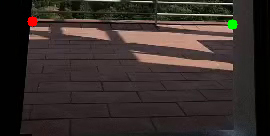
\includegraphics[width=0.3\linewidth]{img/two_points.jpg}
\end{center}
   \caption{In this window the user has selected only two points so far; an error message will be displayed in the terminal if he or she presses \lstinline{ENTER} before selecting the remaining two.}
\label{fig:twopoints}
\end{figure}

\begin{figure}[H]
\begin{center}
    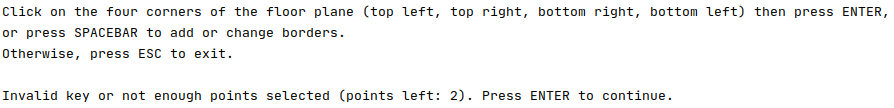
\includegraphics[height=0.122\linewidth]{img/points_terminal.png}
\end{center}
   \caption{An example of the error message displayed in the terminal if the user presses \lstinline{ENTER} before selecting all four corners; the program will not crash, but wait for the remaining mouse clicks.}
\label{fig:pointsterminal}
\end{figure}


%---------------------------------

\subsection{Overlay generation and application}
\label{chap:overlay}
The \lstinline{overlay.py} script contains the \lstinline{generate_overlay()} and \lstinline{apply_overlay()} functions previously mentioned in sections \ref{chap:processframefirst} and \ref{chap:processframe}. Unlike in earlier paragraphs, where the status bar also included the map, in this section a distinction will be made between the words \textit{map}, which is going to designate the actual map generated by the program, and \textit{status bar}, which is going to denote only the grey bar containing the informative text.

\subsubsection{\textit{generate\_overlay()}}
\label{chap:genoverlay}
The \lstinline{generate_overlay()} function begins by defining the maximum map dimensions, determined from the video resolution; the map will have the same width as the frame width minus the minimum status bar width\footnote{The status bar has a minimum width of 200 pixels, needed in order to correctly fit all text.}, while its maximum height is calculated according to a specified percentage of the frame height, that can be found in the \lstinline{INI} file.

The function proceeds with calling what is probably the single most important operation in the program, namely the \lstinline{warp()}\footnote{Defined in the homonymous Python script.} method that executes the homography and returns the transformation matrix and warped image (the latter is going to be resized into the actual map).

At this point \lstinline{generate_overlay()} checks if said image is larger than the maximum map dimensions calculated in the beginning, and proceeds to scale it accordingly, then eventually adds a horizontal border if the resulting height is smaller than the status bar height (see fig. \ref{fig:hormap} and \ref{fig:vermap}).

\begin{figure}[H]
  \centering
  \begin{minipage}[b]{0.45\textwidth}
    \centering
    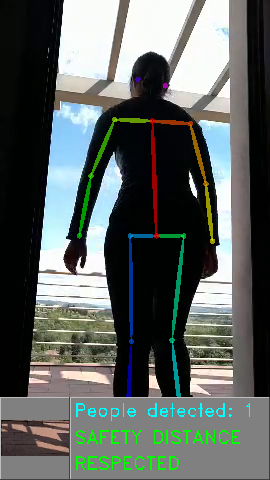
\includegraphics[height=7cm,keepaspectratio]{img/horizontal_map.jpg}
    \caption{Horizontal map with top and bottom borders.}
    \label{fig:hormap}
  \end{minipage}
  \hfill
  \begin{minipage}[b]{0.45\textwidth}
    \centering
    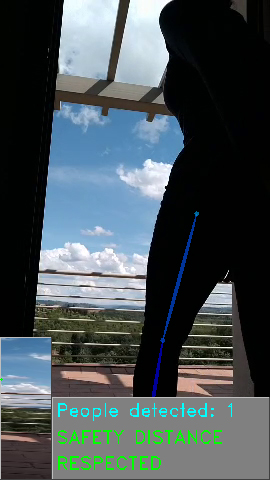
\includegraphics[height=7cm,keepaspectratio]{img/vertical_map.jpg}
    \caption{Dummy vertical map (shows how the GUI handles it).}
    \label{fig:vermap}
  \end{minipage}
\end{figure}

In order to have a flexible overlay that will not impede a correct visualization of the scene after its application, the map and status bar can assume a total of four different positions on the video, as shown in figures \ref{fig:ovl0}, \ref{fig:ovl1}, \ref{fig:ovl2} and \ref{fig:ovl3}.

\begin{figure}[H]
  \centering
  \begin{minipage}[b]{0.45\textwidth}
    \centering
    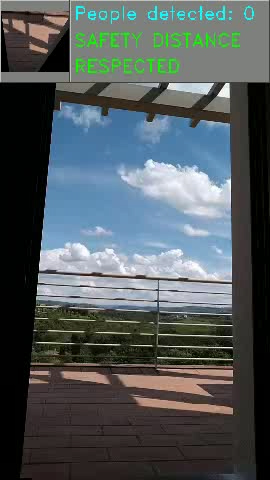
\includegraphics[height=6cm,keepaspectratio]{img/ovl_0.jpg}
    \caption{Status bar with overlay position n\textdegree 0.}
    \label{fig:ovl0}
  \end{minipage}
  \hfill
  \begin{minipage}[b]{0.45\textwidth}
    \centering
    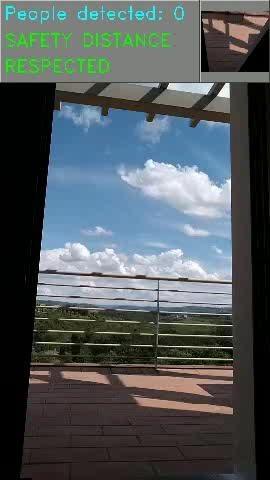
\includegraphics[height=6cm,keepaspectratio]{img/ovl_1.jpg}
    \caption{Status bar with overlay position n\textdegree 1.}
    \label{fig:ovl1}
  \end{minipage}
\end{figure}

\begin{figure}[H]
  \centering
  \begin{minipage}[b]{0.45\textwidth}
    \centering
    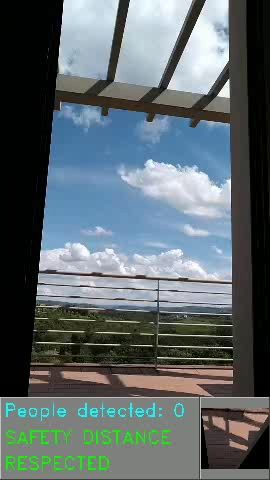
\includegraphics[height=6cm,keepaspectratio]{img/ovl_2.jpg}
    \caption{Status bar with overlay position n\textdegree 2.}
    \label{fig:ovl2}
  \end{minipage}
  \hfill
  \begin{minipage}[b]{0.45\textwidth}
    \centering
    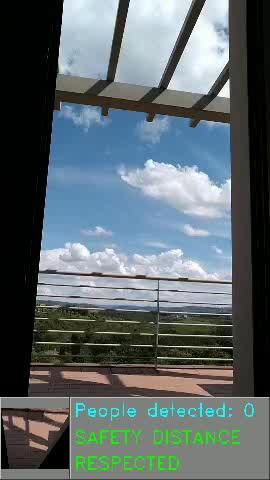
\includegraphics[height=6cm,keepaspectratio]{img/ovl_3.jpg}
    \caption{Status bar with overlay position n\textdegree 3.}
    \label{fig:ovl3}
  \end{minipage}
\end{figure}

The next operations add a thin border\footnote{Its thickness can actually be defined in the setup file.} around the map and status bar as a graphical improvement and compute their corners according to the chosen overlay position. This information, together with a few other parameters derived from the \lstinline{warp()} function (among which the homography matrix and final map image), are added to the \lstinline{overlay_data} dictionary alongside the existing parameters read from the setup file. These variables will be used for the application of the overlay in each subsequent frame and to ensure the correct processing of the keypoints returned by the OpenPose library since, as seen, the map is not just a simple homography of the first video frame, but undergoes a series of resizings in order to adapt it to the overlay itself.

\subsubsection{\textit{apply\_overlay()}}
\label{chap:apploverlay}
This function, as its name implies, applies an existing map and its status bar to each frame of the video. By using the \lstinline{overlay_data} dictionary read from the \lstinline{INI} file and updated after the overlay generation, together with the data about the people’s position calculated within the two \lstinline{process_frame} functions, it draws the map, status bar and informative text over each video frame according to the data it receives.

It is worth noting that this function further adjusts the calculated position of the people returned by \lstinline{transform_coords()} by calling on this data the \lstinline{adjust_position()} function\footnote{Found in the \lstinline{transform_coords.py} script.}, in order to draw the coloured dots consistently with the map position (which, as specified in section \ref{chap:genoverlay}, can be in any of the four corners of the frame). This method also uses a tolerance\footnote{Specified, in pixels, in the \lstinline{INI} file.} to enable the program to draw on the edge some points that fall not too far outside the map, a feature needed in those cases where OpenPose returns keypoints slightly off the real position of the person they refer to (for example when the person lifts a foot, see fig. \ref{fig:edge}).

\begin{figure}[H]
\begin{center}
    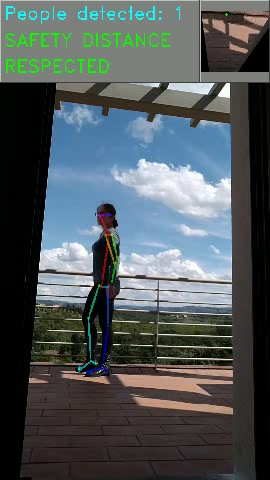
\includegraphics[height=0.55\linewidth]{img/edge.jpg}
\end{center}
   \caption{In this particular frame the estimated position of the person would fall slightly outside the top edge of the map (around 5 or 6 pixels from the edge); her position is nonetheless displayed correctly because a tolerance of 20 pixels has been set in the setup file.}
\label{fig:edge}
\end{figure}

%---------------------------------

\subsection{Homography}
\label{chap:homography}

A homography is a perspective transformation of a plane, that is, a reprojection of a plane from one view into another\cite{homography}. It has many practical applications in computer vision, such as image rectification, image registration, or computation of camera motion - rotation and translation - between two images \cite{homographywiki}.

The homography matrix $H$ is a $3\times 3$ matrix that relates two points on different planes as follows\cite{cvhomography}:

\begin{equation}
    \begin{bmatrix}
    x \\
    y \\
    1 \\
    \end{bmatrix}
    = 
    H
    \begin{bmatrix}
    x' \\
    y' \\
    1
    \end{bmatrix}
    =
    \begin{bmatrix}
    h_{00} & h_{01} & h_{02} \\
    h_{10} & h_{11} & h_{12} \\
    h_{20} & h_{21} & h_{22}
    \end{bmatrix}
    \begin{bmatrix}
    x' \\
    y' \\
    1
    \end{bmatrix}
\end{equation}

In other words, given a point with coordinates $(x, y)$ in the source image, $H$ allows to calculate the coordinates $(x', y')$ of the corresponding point in the destination (projected) image\footnote{The destination image could simply be a different view of the scene represented in the source image, as shown in figure \ref{fig:corrpoints}.}; if applied to the whole source image, that is to every source point, the homography matrix returns the destination image in its entirety.

In order to be able to use it, however, one needs to first compute $H$; the simplest way to do this is to use the coordinates of at least four corresponding points (points that lie on the same plane but are viewed from a different perspective, see fig. \ref{fig:corrpoints}): $\{(x_0, y_0), (x_1, y_1), (x_2, y_2), (x_3, y_3)\}$ and $\{(x_0', y_0'), (x_1', y_1'), (x_2', y_2'), (x_3', y_3')\}$.

The importance of the source and destination points, extensively discussed in sections \ref{chap:srcpts}, \ref{chap:corners} and \ref{chap:points}, is now clear since the OpenCV library provides a useful function to calculate a homography matrix given these corners, namely \lstinline{findHomography()}; the matrix returned by this method can be subsequently used to transform any other point in the source image, and as further explained is the basis for this program's map creation and estimation of the people's position.

\begin{figure}[H]
\begin{center}
    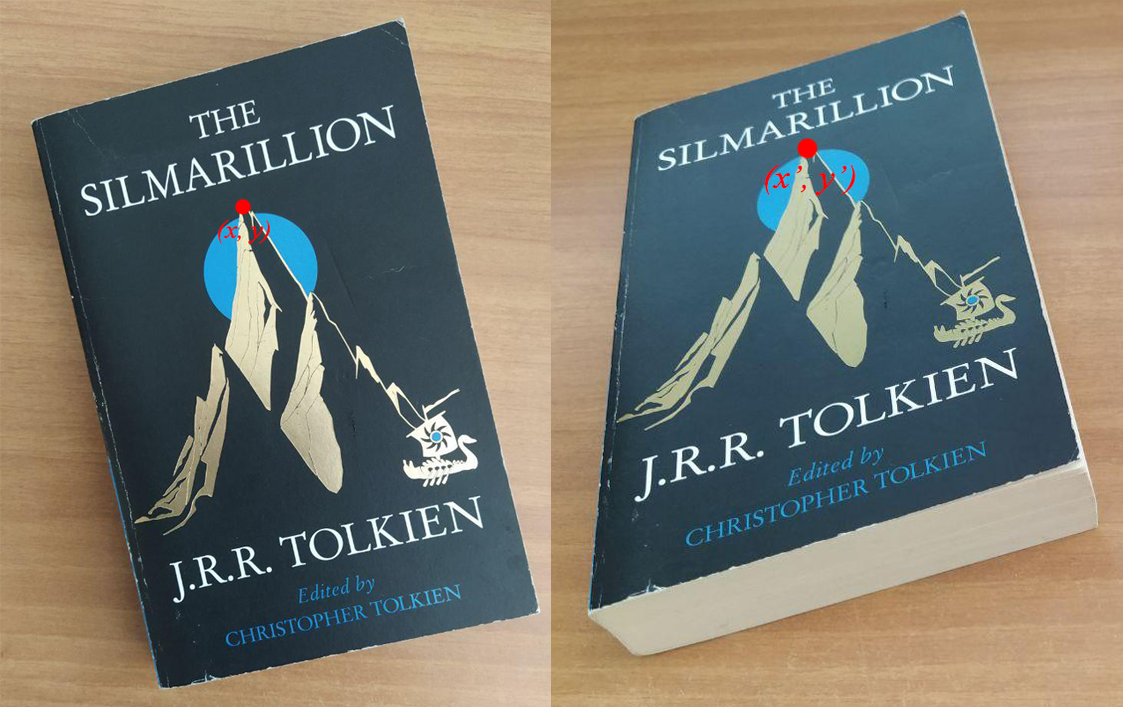
\includegraphics[height=0.6\linewidth]{img/corrpoints.jpg}
\end{center}
   \caption{An example of corresponding points in the source image (left) and destination image (right).}
\label{fig:corrpoints}
\end{figure}

\subsubsection{\textit{warp()}}
\label{chap:warp}
As mentioned earlier, the \lstinline{warp()} function executes the actual geometric transformation needed to obtain the map from the original video frame, along with the data further needed by the \lstinline{generate_overlay()} method in order to create a valid overlay. Its functionality depends on whether the user has chosen to use floor or mat reference points, but can be outlined in both cases with the following steps:

\begin{enumerate}
\item \footnote{Floor case only.}Check if destination points are available (see section \ref{chap:map}); if they are, go to step 3;
\item Generate destination points;
\item Get homography matrix using the OpenCV \lstinline{findHomography()} function;
\item \footnote{Mat case only.\label{matnote}}Translate the homography matrix in order to apply it to the whole frame; this step is needed because otherwise the \lstinline{warpPerspective()} function would crop an essential part of the original frame\cite{cvcrop} (see fig. \ref{fig:chessmap} and \ref{fig:chessmapcropped} for an example); $t_{02}$ and $t_{12}$ are set according to the original image width and height:
\begin{equation}
    H' = T
    \begin{bmatrix}
    h_{00} & h_{01} & h_{02} \\
    h_{10} & h_{11} & h_{12} \\
    h_{20} & h_{21} & h_{22}
    \end{bmatrix}
    =
    \begin{bmatrix}
    1 & 0 & t_{02} \\
    0 & 1 & t_{12} \\
    0 & 0 & 1
    \end{bmatrix}
    \begin{bmatrix}
    h_{00} & h_{01} & h_{02} \\
    h_{10} & h_{11} & h_{12} \\
    h_{20} & h_{21} & h_{22}
    \end{bmatrix}
\end{equation}
\item Apply homography to the original video frame using the OpenCV \lstinline{warpPerspective()} function;
\item \footref{matnote}Crop the warped image to contain only the region of interest; this operation is needed because the previous translation causes the homography to be applied to the whole frame, of which only the mat and a given region of interest around it is actually needed for the map.
\end{enumerate}

\begin{figure}[H]
  \centering
  \begin{minipage}[b]{0.45\textwidth}
    \centering
    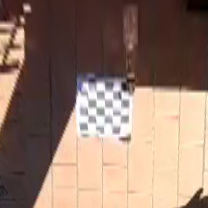
\includegraphics[height=4cm,keepaspectratio]{img/chess_map.jpg}
    \caption{Correct map of the requested region of interest generated from mat corners after having translated the homography matrix.}
    \label{fig:chessmap}
  \end{minipage}
  \hfill
  \begin{minipage}[b]{0.45\textwidth}
    \centering
    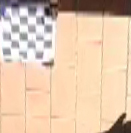
\includegraphics[height=4cm,keepaspectratio]{img/chess_map_cropped.jpg}
    \caption{Cropped map generated from the same mat corners by the \lstinline{warpPerspective} function if the homography matrix is not translated.}
    \label{fig:chessmapcropped}
  \end{minipage}
\end{figure}

For debug purposes, the warped image (which is different from the final map because, as previously seen, more resizing occurs in the \lstinline{generate_overlay()} function) can be shown if a parameter \lstinline{show = True} is passed to \lstinline{warp()}. However, sometimes this image would be too big to fit the screen, so the program automatically resizes it according to the display resolution that is detected through the \lstinline{screeninfo} library\cite{screeninfo}.

The script finally returns the warped image and the homography matrix (the translated version in the mat case), along with the parameters needed for the subsequent transformations (namely, in the mat case, an offset introduced by the translation and the map dimensions in centimeters, which have been automatically calculated from the mat's own dimensions).

%---------------------------------

\subsection{People’s position estimation}
\label{chap:position}

Both \lstinline{process_frame} functions use an external script to obtain and process the people’s position, specifically the \lstinline{transform_coords.py} script. This program takes in input the OpenPose keypoints along with the homography matrix and other variables calculated by the \lstinline{generate_overlay()} function (that are needed to ensure consistency with the subsequent transformations that the original warped image undergoes in the same function), and returns an array containing the pixel coordinates of each person detected in the frame along with the distance (in centimeters) between each of them.

The program is quite simple: after getting the average position of the two heel keypoints of each person\footnote{OpenPose keypoints number 21 and 24 for the BODY\_25 model\cite{opkp}}, it applies the homography matrix to them by using the OpenCV \lstinline{perspectiveTransform()}\cite{cvpertrans} function along with any offsets generated by the homography translation (only in the mat case). The particular choice of the heels was made in order to exploit the fact that OpenPose can detect even people that might partially fall outside the frame, and can prove effective wherever the floor covers the (almost) entirety of the frame and only the people’s feet are visible in the furthest area (fig. \ref{fig:feet}).

An array containing the previous positions of the same people is used to smooth the transition between one frame and the next by applying the following formula, where $f$ is the number of the current frame and $\alpha$ is a parameter that can be set in the \lstinline{INI} file as the \lstinline{position_alpha} parameter\footnote{It has been observed that $\alpha = 0,90 \sim 0,95$ achieves the desired effect.}:

\begin{equation}
x(f) = \alpha \cdot x(f) + (1-\alpha) \cdot x(f-1)
\label{eq:weightx}
\end{equation}
\begin{equation}
y(f) = \alpha \cdot y(f) + (1-\alpha) \cdot y(f-1)
\label{eq:weighty}
\end{equation}

\begin{figure}[H]
\begin{center}
    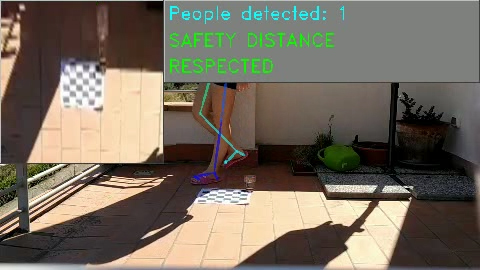
\includegraphics[width=0.8\linewidth]{img/feet.jpg}
\end{center}
   \caption{The person shown in this video is detected by OpenPose even if only the lower half of her body is visible.}
\label{fig:feet}
\end{figure}

The measure was introduced in order to reduce the shaky movement of the position drawn on the map caused by the Openpose library which, as one would expect, does not return sufficiently accurate keypoints for each frame, even if the person moves by only a few pixels.

This feature is however limited by the fact that the program does not distinguish between different people, so therefore it only works if OpenPose detects the same number of people between frames and returns them in the same order. In fact, it has been noted that OpenPose \textit{does not} return detected people always in the same order, and this caused noticeable errors in the map position drawing. This complication has been solved in the following naive, yet in practice rather effective way: before applying equations \ref{eq:weightx} and \ref{eq:weighty}, the array containing the people's positions is reordered by sorting the $x$ coordinates (each of them together with their relative $y$ coordinate) in ascending order. Since a person's position does not usually change too much from a single frame to another, this approach ensures that every position stored in the sorted array corresponds to the same person, every time.

The \lstinline{transform_coords.py} file also contains a few auxiliary functions, namely \lstinline{adjust_position()} (used in \lstinline{apply_overlay()}, see section \ref{chap:apploverlay}) and \lstinline{get_distance()}, needed to calculate the distance between each pair of people detected in each frame and warn about any violations.

%---------------------------------

\subsection{Practical measures for a real-world application}
\label{chap:realworld}
As stated in the abstract of this paper, there have been taken multiple measures in order to create a program less prone to error and ensure an overall smooth user experience.

Even if these technicalities are best observed directly in the code, a few of them are hereby mentioned as a sample of this effort to limit various errors:
\begin{itemize}
    \item all parts of the program where user input is required are heavily foolproofed against invalid input, mouse corner selection included (as mentioned in \ref{chap:points});
    \item in the \lstinline{physical_distance_detector.py} script, the destination name that the user can enter as a command line argument has its extension analysed and corrected if absent or wrong (in the current configuration the OpenCV library can only save videos in the \lstinline{AVI} format);
    \item various readable errors are printed in the terminal window if some of the parameters found in the setup file are out of their range, such as the overlay position and the floor/mat source points;
    \item as seen in the \lstinline{warp()} function (section \ref{chap:warp}), a whole block of code is devoted to checking that the warped image is not larger than the current screen resolution (on either Windows or Linux), and if so, to resizing said image accordingly; this has been implemented as a measure to avoid enormous windows on small screens (such as those that are usually found in surveillance systems, a possible real-world application of this software).
\end{itemize}


%-------------------------------------------------------------------------

\section{System requirements}
\label{chap:requirements}
The system requirements for this software are mainly derived from the demanding requirements of the OpenPose library which, as stated in the official documentation for the NVIDIA GPU version, are the following\cite{opprereq}\cite{opreq}:

\begin{itemize}
    \item CMake GUI\cite{cmake};
    \item NVIDIA graphics card with at least 1.6 GB memory available;
    \item CUDA 10 (for Ubuntu 18)\cite{cuda}
    \item at least 2.5 GB of free RAM memory for BODY\_25 model (assuming cuDNN installed);
    \item highly recommended: cuDNN 7.5 (for Ubuntu 18)\footnote{It has been observed, on this project's development system (see \ref{chap:specs}), that the OpenPose library quickly runs out of memory without cuDNN installed, so in this case this requirement one turned out to be actually \textit{highly necessary}.};
    \item highly recommended: a CPU with at least 8 cores.
\end{itemize}

The Caffe dependency is automatically satisfied when downloading the OpenPose source code (which contains it), while all other libraries (OpenCV, numpy\cite{numpy}, screeninfo) can be easily installed using the \lstinline{pip3} command on both Linux and Windows.

%---------------------------------

\subsection{OpenPose installation}
\label{chap:install}
A whole new paper could be written about the difficulties encountered while installing the necessary requirements for the OpenPose library, but since this is not the purpose of this article, only a brief summary is hereby given in order to inform the user about the possible complications that might arise while trying to compile OpenPose from its source code\cite{opinstall}\cite{opinstallunoff}.

\subsubsection*{Windows 10 + AMD graphics}
\label{chap:win10amd}
An early intention for this project was to develop it on Windows 10 using an AMD Radeon Vega 64 GPU, which was among the few AMD GPUs supported by OpenPose\cite{opprereqwin}; however, after intensive trials, this turned out to be infeasible as the OpenPose library kept throwing CUDA errors in spite of the system having no NVIDIA graphics card mounted on board. It has been speculated that this problem arised from the fact that the machine did use, at a certain point in its life, a NVIDIA GPU, and although that had been long uninstalled together with its drivers\footnote{The removal of all NVIDIA drivers, CUDA and cuDNN software has been accomplished using the official NVIDIA guides and uninstallers which, as stated in this paragraph, seem to actually be insufficient to restore the machine to its previous state. Ulterior research and troubleshooting, even outside of the official NVIDIA channels, did not help in this matter.}, some traces of the previous installation have probably remained somewhere in the Windows environment and caused OpenPose to believe that it was running on a CUDA system – which it was not.
In spite of all the efforts, it has not been possible to completely eradicate these remains without resorting to highly invasive methods (such as reinstalling Windows), which were not an option.

\subsubsection*{Windows 10 + NVIDIA graphics}
\label{chap:win10nvidia}
The subsequent approach hoped to solve the detection of nonexistent NVIDIA drivers by reinstalling them again and actually using a NVIDIA GPU. Many official\cite{cudaofficialwin} and unofficial\cite{cudaunofficial} guides have been followed\footnote{The author has read so much material on the subject that it is unthinkable to account for all of it in this paper, even if only for the fact that after a certain point it was impossible to keep trace of all procedures that had been tried; none of it, in any case, solved the problem.} in order to properly reinstall these drivers but, notwithstanding the efforts, CUDA kept throwing the same error as before. Given that much time had already been invested in these attempts, the author thus deemed counterproductive (see fig. \ref{fig:meme}) to keep trying without first reinstalling Windows 10, and since this was not possible, a new boot partition has been created in order to move the project’s development on Linux.

\begin{figure}[H]
\begin{center}
    
\includegraphics[width=0.3\linewidth]{img/meme.png}
\end{center}
   \caption{This hilarious meme\cite{meme} pretty much sums up the author's reaction after more than a week of attempts to get OpenPose to work on Windows 10. Funnily enough, Ubuntu proved not much better - at least initially.}
\label{fig:meme}
\end{figure}

\subsubsection*{Ubuntu 18.04 + NVIDIA graphics}
\label{chap:ubuntu}
Using a clean Linux installation was supposed to facilitate the process of installing the requirements for OpenPose; it turned out that even on Linux, NVIDIA software was still very challenging to install.

The main problem was to be able to get a compatible GPU driver to work with CUDA and vice versa, because they kept conflicting during their own installations even if, according to official documentation\cite{cudaofficiallinux}, they were supposed to get along just fine. cuDNN also posed a problem, and extensive research was needed in order to get CUDA to find it; for the purpose of installing this library, one should be able to confidently read and modify CMake files\cite{cudnnnotfound}.

After much trial and error, troubleshooting and scouring of the most remote forum posts, a working configuration has been obtained after compiling the OpenPose source code\cite{opcompile}\cite{opquick}; however, given the tremendous amount of attempts and software installed\footnote{It has been estimated that about 15 GB of data have been downloaded in order to install, uninstall and reinstall the NVIDIA software with all its requirements  - more than once - until everything worked as was supposed to.}, writing a complete guide about this process would be quite problematic and possibly useless, since there are too many dependencies among all the packages that had to be installed and they are continuously updated, thus generating new incompatibilities.

%---------------------------------

\subsection{System specifications}
\label{chap:specs}
This project has been developed and tested on a system with the following specifications:
\begin{itemize}
    \item \textbf{Motherboard}: MSI MS-B106
    \item \textbf{CPU}:  Intel Core i7-6700K @ 4.01 GHz
    \item \textbf{RAM}: 16 GB DDR4 @ 3000 MHz
    \item \textbf{GPU (AMD)}: AMD Radeon Vega 64 \textit{(later replaced with the NVIDIA GPU)}
    \item \textbf{GPU (NVIDIA)}: Zotac GeForce GTX 970 \textit{(courtesy of the University of Florence)}
    \item \textbf{SSD}: Samsung SSD 850 EVO $[$500 GB$]$
    \item \textbf{HDD}: WD Blue $[$3 TB$]$
    \item \textbf{OS}: Ubuntu 18.04.4 LTS (Bionic Beaver)
    \item \textbf{NVIDIA driver}: v. 440.100
    \item \textbf{CUDA}: v. 10.2
    \item \textbf{cuDNN}: v. 7.6.5
\end{itemize}

%-------------------------------------------------------------------------

\section{Conclusions}
\label{chap:conclusions}
The software here presented is able to determine the physical distance between people with satisfying accuracy (around $\pm 5-15 cm$), and in contrast to other similar programs\cite{others} it also draws a map of the environment where it marks the position of every person. It is uniquely based entirely on geometrical transformations and relies on OpenPose, a solid pose estimation library. Even though the latter represented a great challenge to configure, it resulted to be a complete and easy to implement tool once it was properly working.

%---------------------------------

\subsection{Future developments}
\label{chap:future}
The project fully achieves its purpose while introducing new mechanics along the way. In spite of the effort put in making it as complete as possible, however, there is certainly room for improvement; many exceptions, for example, have not been covered (especially some niche errors thrown by the OpenPose and OpenCV libraries), and although the code has been fully refactored before the final commit, it could probably be further optimized for a faster execution.

OpenPose's keypoints could be further elaborated in order to get better positions. However, as the author has observed while working on the position smoothing part (discussed in \ref{chap:position}), the last improvement would require a lot of comparisons between frames and much additional data should be saved for each frame, and together these operations would greatly reduce overall performance because of the number of calculations that such processing would require for every single video frame.

In the hopes that the final user will not come across these untested exceptions nor will try to run the program on low-end systems, the source code remains available at the project's original repository\cite{repo} for someone else to read and eventually work on.

%-------------------------------------------------------------------------

\bibliographystyle{plain}
\bibliography{refs}

%-------------------------------------------------------------------------

\vspace{3cm}

\begin{figure}[H]
\begin{center}
    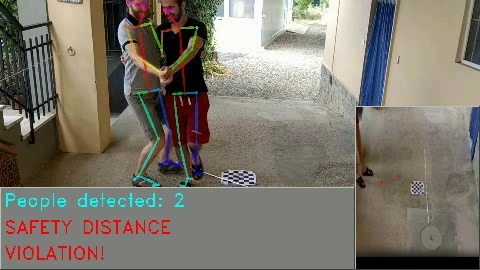
\includegraphics[width=0.85\linewidth]{img/sample_c3.jpg}
\end{center}
   \caption{Despite repeatedly violating the safety distance (of course, for research purposes), these test subjects (Marco \& Riccardo Pratelli) had their share of fun while recording the sample videos. The author kindly thanks them for their contribution.}
\label{fig:c3}
\end{figure}

%-------------------------------------------------------------------------

\end{document}